\documentclass[titlepage,usenames,a4,landscape,semhelv]{seminar}
\newcommand{\presenter}{Abram Hindle}
\newcommand{\conference}{}
\newcommand{\gettitle}{Temporal Developer Concept Witchery: Latent Dirichlet Allocation Applied to Revisions}

\newcommand{\gettitleproper}{\gettitle}
\newcommand{\names}{Abram Hindle, Micheal W. Godfrey, Richard C. Holt}
\author{
\names \\ 
{\small Software Architecture Group }\\
\small David R. Cheriton School of Computer Science\\
\small University of Waterloo\\
\small Canada\\
ahindle@cs.uwaterloo.ca
}



%%% Local Variables: 
%%% mode: latex
%%% TeX-master: t
%%% End: 

\usepackage{xspace,verbatim,listings}
\newcommand{\clstinline}[1]{\lstinline[language=c]!#1!}
\usepackage{graphicx}
\usepackage{comment}
%\usepackage[breaklines]{listings}
\usepackage{seminar}
\usepackage[usenames]{color} 
%\usepackage[pdftex]{color}
\usepackage{hyperref}
\input{seminar.bug}
\input{seminar.bg2}
\usepackage{tabularx}
\usepackage{fancyhdr}

\usepackage{graphicx}
\usepackage{amsmath}
\usepackage{amsfonts}
\usepackage{amssymb}
\usepackage{comment}
\usepackage{rotating} 
\usepackage{xspace}


\newcommand{\igh}[1]{
  \centering
  \includegraphics[height=0.9\textheight]{#1}
}
\newcommand{\igbigh}[1]{
  \centering
  \includegraphics[height=1.1\textheight]{#1}
}

\newcommand{\igwh}[1]{
  \includegraphics[width=0.4\textwidth]{#1}
}


\newcommand{\igw}[1]{
  \centering
  \includegraphics[width=0.9\textwidth]{#1}
}

\newcommand{\igws}[1]{
  \includegraphics[width=0.8\textwidth]{#1}
}

%WARNING THIS DOES A \newslide
% \renewcommand{\slideleftmargin}{-#1cm}        
\newcommand{\shiftleft}[2]{
        \newslide
        \renewcommand{\slideleftmargin}{-#1cm} 
        #2
        \newpage
        \leftmargin{0cm}
        \renewcommand{\slideleftmargin}{5mm}
}


\slidesmag{6}

\noxcomment
  \renewcommand{\slidetopmargin}{15.5mm}
  \renewcommand{\slidebottommargin}{13mm}
%  \renewcommand{\slidetopmargin}{15.5mm}
%  \renewcommand{\slidebottommargin}{13mm}

%  \renewcommand{\slideleftmargin}{0mm}
%  \renewcommand{\slideleftmargin}{-1cm}
\newcommand{\bitem}[1]{\item {\bf #1}: }
  %\renewcommand{\sliderightmargin}{1cm}
\newcommand{\catfile}[1]{ \newslide {\bf #1} 
	{\scriptsize 
		\tt 
		\lstinputlisting[language=PERL,breaklines=true]{#1} 
	} 
}
\newcommand{\sslide}[1]{ \newslide
	{\huge\bf #1}
}
\newcommand{\ttt}[1]{
	``{\tt #1}''
}





\title{\large \gettitleproper}
\renewcommand{\thetitle}{\gettitle}
\newcommand{\listperl}[1]{
	{\scriptsize
		\tt
	\lstinputlisting[language=PERL,breaklines=true]{#1}
	}
}
\newcommand{\listidl}[1]{
	{\scriptsize
		\tt
	\lstinputlisting[language=IDL,breaklines=true]{#1}
	}
}
\newcommand{\hrf}[1]{
	\href{#1}{#1}
}
%\newenvironment{notes}[0]{\tt \begin{note}}{ \end{note}  }

\newcommand{\softChange}{\textsf{softChange}\ }
\newcommand{\igColumnReal}[1]{\includegraphics[width=.9\textwidth]{#1}}
\newcommand{\igReal}[1]{\includegraphics[width=.9\textwidth]{#1}}
\markboth{ }{\presenter \thesection }

\newcommand{\albertaCVS}{\textsf{JReflex}\ }

% \fancyfoot[L]{\tiny \presenter}
% \fancyhead[L]{ \tiny \bf \gettitle}
% \fancyhead[R]{ \tiny \conference}
% \fancyfoot[R]{\tiny \thepage}

\newcommand{\fancyfootl}{\tiny \presenter}
\newcommand{\fancyheadl}{\tiny \bf \gettitle}
\newcommand{\fancyheadr}{\tiny \conference}
\newcommand{\fancyfootr}{\tiny \thepage}



\newcommand{\fancyempty}{
\renewcommand{\headrulewidth}{1.0mm}
\renewcommand{\footrulewidth}{0pt}
\fancyfoot[L]{}
\fancyfoot[R]{}
\fancyhead[L]{\fancyheadl}
\fancyhead[R]{\fancyheadr}
\renewcommand{\slidetopmargin}{15.5mm}
\renewcommand{\slidebottommargin}{13mm}
\renewcommand{\slidetopmargin}{0.5cm}
\renewcommand{\slidebottommargin}{3.0cm}
\renewcommand{\headsep}{0.0cm}
\renewcommand{\slideleftmargin}{5mm}
\renewcommand{\sliderightmargin}{0cm}

}
\newcommand{\fancyfancy}{
\renewcommand{\headrulewidth}{1.0mm}
\renewcommand{\footrulewidth}{1.0mm}
\fancyfoot[L]{\fancyfootl}
\fancyhead[L]{\fancyheadl}
\fancyhead[R]{\fancyheadr}
\fancyfoot[R]{\fancyfootr}
\renewcommand{\slidetopmargin}{15.5mm}
\renewcommand{\slidebottommargin}{13mm}
\renewcommand{\slidetopmargin}{0.5cm}
\renewcommand{\slidebottommargin}{0.5cm}
\renewcommand{\slideleftmargin}{5mm}
\renewcommand{\sliderightmargin}{0cm}

}

\fancypagestyle{empty}{\fancyempty}
\fancypagestyle{main}{\fancyfancy}

\fancyhf{}
\fancyfancy

\pagestyle{fancy}

\renewcommand{\headrulewidth}{1.0mm}
\renewcommand{\footrulewidth}{1.0mm}


\slideframe{none}
\renewcommand{\headwidth}{\textwidth}
\renewcommand{\slidetopmargin}{0.5cm}
\renewcommand{\slidebottommargin}{0.5cm}


\newcommand{\igH}[1]{\includegraphics[height=.9\textheight]{#1}}
\newcommand{\igHh}[1]{\includegraphics[height=.5\textheight]{#1}}
\newcommand{\igHd}[1]{\includegraphics[height=.8\textheight]{#1}}
\newcommand{\igHq}[1]{\includegraphics[height=.25\textheight]{#1}}

\newcommand{\igW}[1]{}
\newcommand{\igWsixth}[1]{\includegraphics[width=.6\textwidth]{#1}}
\newcommand{\igWseventh}[1]{\includegraphics[width=.6\textwidth]{#1}}

\newcommand{\igWh}[1]{\includegraphics[width=.45\textwidth]{#1}}
\newcommand{\igWt}[1]{\includegraphics[width=.3\textwidth]{#1}}

\newcommand{\igWhalf}[1]{\includegraphics[width=.45\textwidth]{#1}}

\definecolor{source}{rgb}{1.0,0.7,0.0}
\definecolor{test}{rgb}{0.19,0.43,0.53}
\definecolor{build}{rgb}{0.73,0.0,0.50}
\definecolor{documentation}{rgb}{0.38,0.77,0.00}
\definecolor{doc}{rgb}{0.38,0.77,0.00}



\newcommand{\ess}[1]{\texttt{S#1}}
\newcommand{\dee}[1]{\texttt{D#1}}
\newcommand{\bee}[1]{\texttt{B#1}}
\newcommand{\tee}[1]{\texttt{T#1}}
\newcommand{\Apluss}{+}
\newcommand{\Aplus}{+}
\newcommand{\Aminus}{-}
\newcommand{\Aquest}{?}
\newcommand{\Aquestionbox}{?}
\newcommand{\Aequals}{=}
\newcommand{\Aequal}{=}

\newcommand{\hess}[1]{{\color{source}\texttt{S#1}}}
\newcommand{\hdee}[1]{{\color{doc}\texttt{D#1}}}
\newcommand{\hbee}[1]{{\color{build}\texttt{B#1}}}
\newcommand{\htee}[1]{{\bf\color{test}\texttt{T#1}}}

\providecommand{\macro}[2]{}
\renewcommand{\macro}[2]{
\providecommand{#1}{}
\renewcommand{#1}{#2}
}


\macro{\Apluss}{\textcolor[gray]{.80}{$\blacksquare$}}
\macro{\Aequal}{$\square$}
\macro{\Aminus}{\textcolor[gray]{.25}{$\blacksquare$}}

\macro{\Apluss}{{\color{red}{$\nearrow$}}}
\macro{\Aminus}{{\color{blue}{$\searrow$}}}
\macro{\Aequal}{{\color{green}{$\square$}}}
\macro{\Aplus}{\Apluss}

\macro{\Apluss}{{\color{red}{$\blacksquare$}}}
\macro{\Aminus}{{\color{blue}{$\blacksquare$}}}
\macro{\Aequal}{{\color{green}{$\square$}}}
\macro{\Aplus}{\Apluss}

\macro{\Apluss}{{\color{red}{$\blacksquare$}}}
\macro{\Aminus}{{\color{blue}{$\blacksquare$}}}
\macro{\Aequal}{{\color{green}{$\square$}}}
\macro{\Aplus}{\Apluss}
\definecolor{equal}{rgb}{0.9,0.0,0.9}
\macro{\Apluss}{{\color{red}{$\blacksquare$}}}
\macro{\Aequal}{{\color{equal}$\diamond$}}
\macro{\Aminus}{{\color{blue}{$\square$}}}
\macro{\Aplus}{\Apluss}
\macro{\Apluss}{{\color{red}{$\blacktriangleright$}}}
\macro{\Aequal}{{\color{equal}$\blacklozenge$}}
\macro{\Aminus}{{\color{blue}{$\blacktriangleleft$}}}

\providecommand{\questionbox}{}
\renewcommand*{\questionbox}{%
\ensuremath{\mathrel{\vcenter{%\offinterlineskip
\hbox{?}\vskip-1.5ex\hbox{$\square$}}}}}

\renewcommand*{\questionbox}{
\includegraphics[width=0.03\textwidth]{quest}
}

\macro{\Apluss}{{\color{red}{$\blacksquare$}}}
\macro{\Aminus}{{\color{blue}{$\square$}}}
\macro{\Aequal}{{\color{green}{$\boxtimes$}}}
\macro{\Aquest}{{\color{black}{$\questionbox$}}}

\macro{\Apluss}{{\color{red}{$\blacktriangle$}}}
\macro{\Aequal}{{\color{equal}$\square$}}
\macro{\Aminus}{{\color{blue}{$\blacktriangledown$}}}
\macro{\Aplus}{\Apluss}


\macro{\Aminus}{{\color{red}{$\blacktriangle$}}}
\macro{\Aequal}{{\color{equal}$\square$}}
\macro{\Apluss}{{\color{blue}{$\blacktriangledown$}}}
\macro{\Aplus}{\Apluss}
\macro{\Aequals}{\Aequal}

\macro{\Aplus}{\Apluss}


\macro{\Aplus}{\Apluss}




\macro{\esstxt}{\texttt{S}}
\macro{\teetxt}{\texttt{T}}
\macro{\deetxt}{\texttt{D}}
\macro{\beetxt}{\texttt{B}}

\providecommand{\ess}[1]{}
\providecommand{\tee}[1]{}
\providecommand{\dee}[1]{}
\providecommand{\bee}[1]{}
\renewcommand{\ess}[1]{\esstxt #1}
\renewcommand{\tee}[1]{\teetxt #1}
\renewcommand{\dee}[1]{\deetxt #1}
\renewcommand{\bee}[1]{\beetxt #1}

\providecommand{\pess}[1]{}
\providecommand{\ptee}[1]{}
\providecommand{\pdee}[1]{}
\providecommand{\pbee}[1]{}
\renewcommand{\pess}[1]{\ess{#1}}
\renewcommand{\ptee}[1]{\tee{#1}}
\renewcommand{\pdee}[1]{\dee{#1}}
\renewcommand{\pbee}[1]{\bee{#1}}

\macro{\essminus}{\ess{\Aplus}}
\macro{\teeminus}{\tee{\Aplus}}
\macro{\deeminus}{\dee{\Aplus}}
\macro{\beeminus}{\bee{\Aplus}}

\macro{\essplus}{\ess{\Aminus}}
\macro{\teeplus}{\tee{\Aminus}}
\macro{\deeplus}{\dee{\Aminus}}
\macro{\beeplus}{\bee{\Aminus}}

\macro{\essequal}{\ess{\Aequal}}
\macro{\teeequal}{\tee{\Aequal}}
\macro{\deeequal}{\dee{\Aequal}}
\macro{\beeequal}{\bee{\Aequal}}


\macro{\esspos}{\ess{\Aminus}}
\macro{\teepos}{\tee{\Aminus}}
\macro{\deepos}{\dee{\Aminus}}
\macro{\beepos}{\bee{\Aminus}}

\macro{\essneg}{\ess{\Aplus}}
\macro{\teeneg}{\tee{\Aplus}}
\macro{\deeneg}{\dee{\Aplus}}
\macro{\beeneg}{\bee{\Aplus}}

\macro{\deequest}{\dee{\Aquest}}

\macro{\x}{\xspace}

\newcommand{\ctest}{{\color{test} Test}\x}
\newcommand{\csource}{{\color{source} Source}\x}
\newcommand{\cdocumentation}{{\color{documentation} Documentation}\x}
\newcommand{\cbuild}{{\color{build} Build}\x}

\newcommand{\Major}{}
\newcommand{\Minor}{}
\renewcommand*{\Major}{\emph{Major}\x}
\renewcommand*{\Minor}{\emph{Minor}\x}

\newcommand{\transition}[2]{
}

\newcommand{\STD}{STD\xspace}
\newcommand{\ISTD}{ISTD\xspace}
\newcommand{\LSTD}{LSTD\xspace}
\newcommand{\VAR}{VAR\xspace}
\newcommand{\IVAR}{IVAR\xspace}
\newcommand{\LVAR}{LVAR\xspace}
\newcommand{\MED}{MED\xspace}
\newcommand{\IMED}{IMED\xspace}
\newcommand{\LMED}{LMED\xspace}
\newcommand{\AVG}{AVG\xspace}
\newcommand{\IAVG}{IAVG\xspace}
\newcommand{\LAVG}{LAVG\xspace}
\newcommand{\SUM}{SUM\xspace}
\newcommand{\ISUM}{ISUM\xspace}
\newcommand{\LSUM}{LSUM\xspace}
\newcommand{\LOC}{LOC\xspace}
\newcommand{\maintainability}{177741}
\newcommand{\cyclomatic}{mccabe}
\newcommand{\mccabe}{mccabe}
\newcommand{\halstead}{Halstead}
\newcommand{\mcc}{MCC\xspace}
\newcommand{\MCC}{MCC\xspace}
\newcommand{\HEFFORT}{HEFFORT\xspace}
 \newcommand{\HVOL}{HVOL\xspace}
\newcommand{\HDIFF}{HDIFF\xspace}
\newcommand{\HLEN}{HLEN\xspace}
\newcommand{\HVOCAB}{HVOCAB\xspace}

\newcommand{\igWsb}[1]{\noindent \includegraphics[width=1.0\textwidth]{#1}}
%\newcommand{\igWsb}[1]{\noindent \includegraphics[scale=1.5,origin=c]{#1}}
\usepackage{wrapfig}

\newenvironment{uquote}
{\list{}{\rightmargin -5em
         \leftmargin  -5em}
\item\relax}
{\endlist}


\newenvironment{uuquote}
{\list{}{\rightmargin 0em
         \leftmargin  0em}
\item\relax}
{\endlist}


\newcommand{\igbigslide}[1]{
\begin{uquote}
\newpage
%\centerslidesfalse
\fancyempty
\noindent
\begin{center}
\includegraphics[width=1.25\textwidth]{#1}
\end{center}
\newpage
\fancyfancy
%\centerslidestrue
\end{uquote}
}

\newcommand{\igbigslidecap}[2]{
\begin{uquote}
\newpage
%\centerslidesfalse
\fancyempty
\noindent
\begin{center}
\includegraphics[width=1.25\textwidth]{#1}
#2
\end{center}
\newpage
\fancyfancy
%\centerslidestrue
\end{uquote}
}


\newcommand{\bigslide}[1]{
\begin{uuquote}
\newpage
\centerslidesfalse
\fancyempty
#1
\newpage
\fancyfancy
\centerslidestrue
\end{uuquote}
}


\newcommand{\imageslide}[2]{
\newslide
\includegraphics[width=0.9\textwidth]{#2}
}

\newcommand{\figcaption}[1]{
\begin{center}
#1\\
\end{center}
}


\newcommand{\ig}[1]{\includegraphics{#1}}
%%%%%%%%%%%%%%%%%%%%%%%%%%%%%%%%%%%%%%%%%%%%%%%%%%%%%%%%%%%%%%%%%%%%%%%%%%%%%%%%
\begin{document}
\pagestyle{fancy} %bars..
\begin{slide}

\begin{center}
{\bf \LARGE \gettitleproper }

{\names } 

{\small Software Architecture Group }\\[-.5em]
{\small David R. Cheriton School of Computer Science}\\[-.5em]
{\small University of Waterloo}\\[-.5em]
{\small Canada}\\[-.5em]
{\small http://swag.uwaterloo.ca/}\\
\{ahindle,migod,holt\}@cs.uwaterloo.ca


\end{center}

\sslide{Introduction}
\begin{itemize}
\item Stakeholders want to know what the focus of the last iteration was
\item Evidence of work done at Retrospective meetings
\item Difference between developer opinion and developer commits


\end{itemize}
\sslide{Dictionary}
\begin{itemize}
\item Message - in this a CVS Commit
\item Word Distribution - count of words occuring in a message
\item Topic - a word distribution that is common amongst messages
\item Trend - a topic that re-occurs


\end{itemize}
\sslide{Developer Trends}
\begin{itemize}
\item Trends
	\begin{itemize}
	\item Continuous or repeating topics
	\item Occur over multiple time windows

\end{itemize}
\end{itemize}
\sslide{LDA}
\begin{itemize}
\item Latent Dirichlet Allocation
\item Like Latent Semantic Indexing (LSI)
\item Like ICA/PCA
\item Black box view:
	\begin{itemize}
	\item Input word distributions of messages, 
	\item Output topics consisting of a word distribution and related messages



\end{itemize}
\end{itemize}
\sslide{Topic Clustering }
\begin{itemize}
\item Need to track continuous topics across 
\item Similarity between topics
\item Clusters of the transitive closure of topics with X\% similarity
	\begin{itemize}
	\item Fill flood along similarity, make subsets of everyone who X\% similar to any of their neighbors, make that a cluster

%\newslide

\igonecap{transitiveclosure}{Clustering topics (black dots) by Transitive Closure based on similarity (arcs)}


\end{itemize}
\end{itemize}
\sslide{Topic Similarity}
\begin{itemize}
\item Given 2 topics
	\begin{itemize}
	\item if their top 10 words 
		\begin{itemize}
		\item share X words (7 or more)
			\begin{itemize}
			\item they are similar




%\igbigslidecap{transitiveclosure}{Clustering topics (black dots) by Transitive Closure based on similarity (arcs)}

% \begin{center}
% \includegraphics[width=\textwidth]{transitiveclosure}
% Clustering topics (black dots) by Transitive Closure based on similarity (arcs)
% \end{center}

%\igninetycap{transitiveclosure}{Clustering topics (black dots) by Transitive Closure based on similarity (arcs)}

\newslide

%\igbigcapb{commit-to-topics}{How commits are aggregated into Topics}
\begin{specquotei}
\begin{center}
\noindent
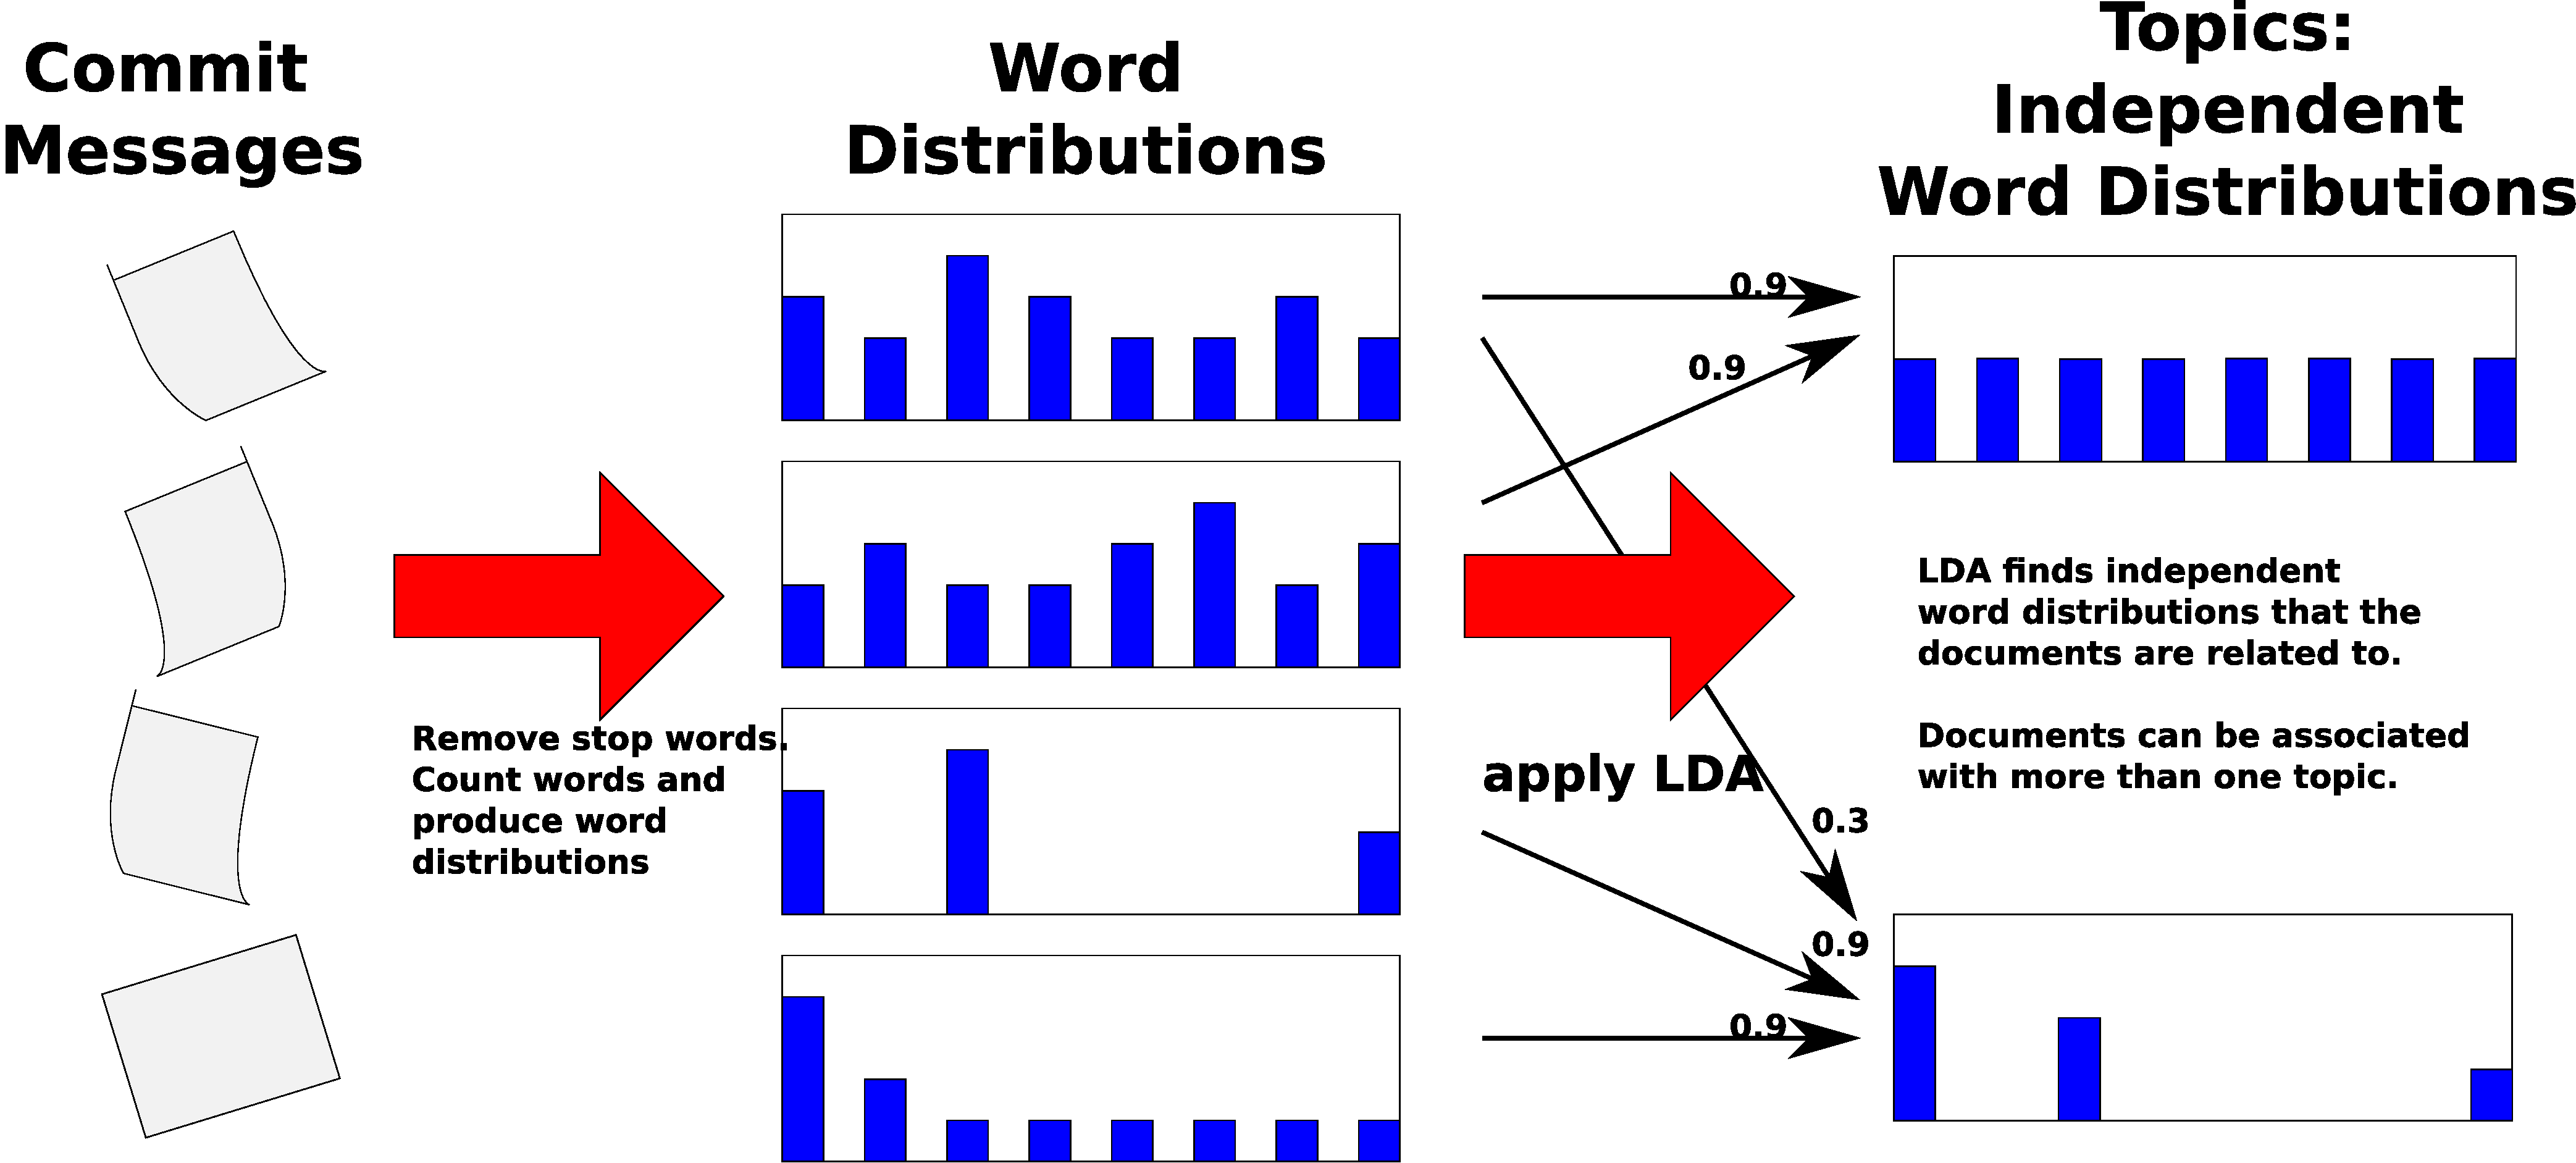
\includegraphics[width=1.25\textwidth]{commit-to-topics} \\
{How commits are aggregated into Topics}
\end{center}
\end{specquotei}

		\end{itemize}
	\end{itemize}
\end{itemize}
\end{itemize}
\sslide{Case Study: Portability}
\begin{itemize}
\item MySQL 3.23 
	\begin{itemize}
	\item Discussions relating to portability
	\item Some topics trends (topics smeared across multiple months)


\newslide

%\begin{table*}
\begin{specquotef}
\centering
\begin{tabular}{|ccc|l|}

%\hline
%2000 &	Jul &	31 &		chmod \\
%2000 &	Sep &	29 &		fixes benchmark logging windows \\
%2000 &	Nov &	28 &		typo fix insert\_multi\_value \\
%2001 &	Jan &	27 &		fixes Innobase Cleanups auto-union \\
%2001 &	Mar &	28 &		2 topics bugfix, logging , TEMPORARY,	\\
\hline
2001 &	Jul &	26 &		update Allow TABLES LOCK [a] \\ 

2001 &	Aug &	25 &		tables row version [a] \\
\hline
%2001 &	Sep &	24 &		update checksum merge \\
%2001 &	Oct &	24 &		fixed fix \\
%2001 &	Dec &	23 &		HPUX SCO fix \\
\hline
2002 &	Feb &	21 &		net buffer length	max\_allowed\_packet [b] \\
2002 &	Mar &	23 &		small buf fix [b]	\\
%\hline
%2002 &	May &	22 &		[popular] fix SCO OSF1 table\_name \\
%2002 &	Nov &	18 &		HPUX11 compiler HP \\
\hline
\hline
2003 &	Feb &	16 &		Linux errno	[c] \\
2003 &	Mar &	18 &		alarm bookmark bug [c] \\
%\hline
%2003 &	Sep &	14 &		Auto logging merge windows distribution fix 64-bit 4.0 Cleanup \\
\hline
\end{tabular} \\
%\caption{Continuous blocks found while tracking topics associated with the word portability in MySQL 3.23}
{Continuous blocks found while tracking topics associated with the word portability in MySQL 3.23}
\label{tab:portability}
%\end{table*}
\end{specquotef}



% \begin{figure}
%	 \centering
%	 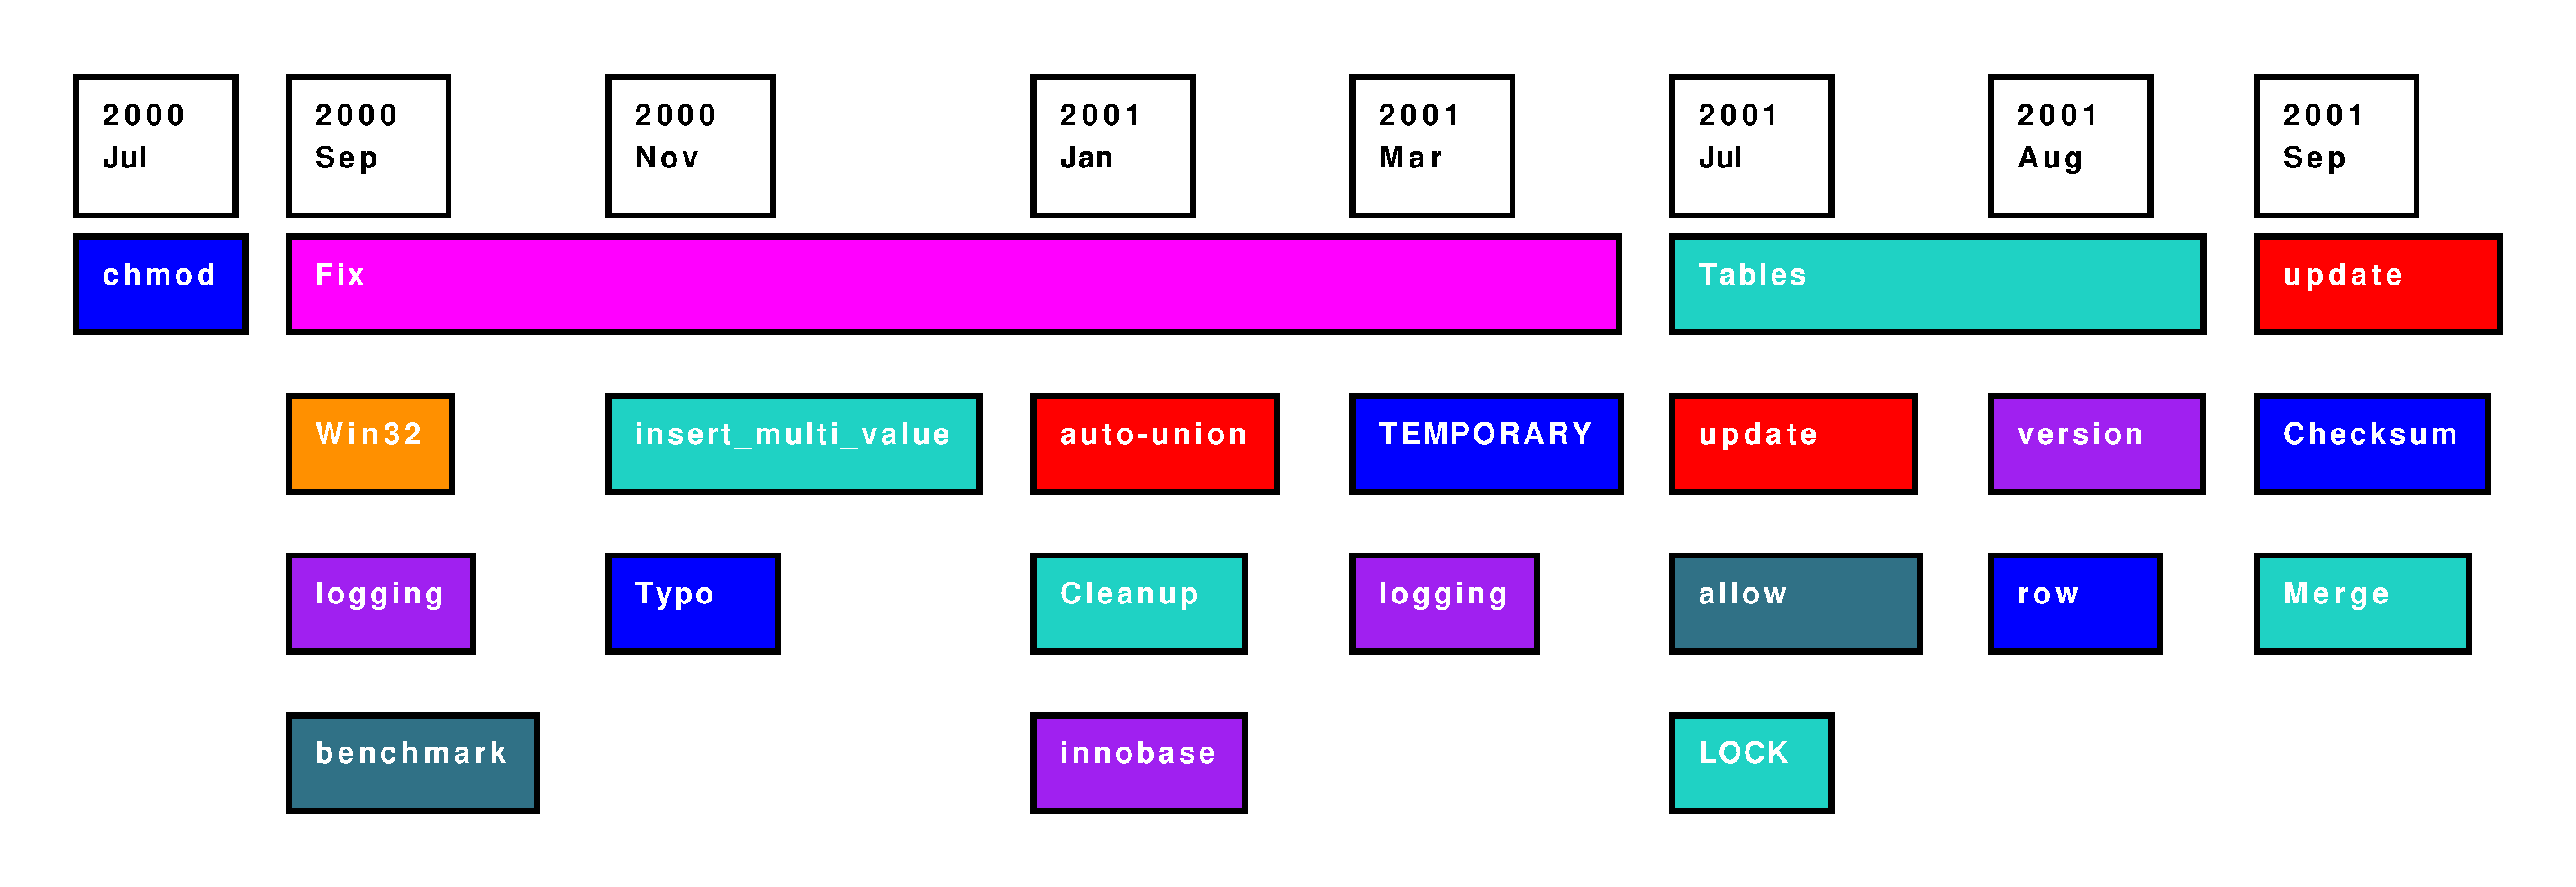
\includegraphics[width=1.5\textwidth]{lda}
%	 \caption{Example of topics extracked from MySQL 3.23}
%	 \label{fig:mysql323}
% \end{figure}

%\igbigslidecap{lda}{Example of topics extracted from MySQL 3.23}
%\igonecap{lda}{Example of topics extracted from MySQL 3.23}
%\igbigcapb{lda}{Example of topics extracted from MySQL 3.23}
%\igbigthirtycapb{lda}{Example of topics extracted from MySQL 3.23}

%\newslide

\igbigthirtyfivecapb{lda}{Example of topics extracted from MySQL 3.23. This is the kind of plot we eventually want to produce: named topics and topic trends}

%\newslide

\end{itemize}
\end{itemize}
\sslide{Case Study: MaxDB 7.500}
\begin{itemize}
\item Autogenerated plots from MaxDB 7.500
\item Multiple Presentations
	\begin{itemize}
	\item Condensed view
	\item Trend Histogram 
	\item Trend View
	\item Trend Timeline


\igbigcap{fixed-time-smear-plot-cropped}{Slice of Topics per Month for MaxDB 7.500}

%\newslide

\igonecap{fixed-time-smear-plot-scaled}{Entire View of Topics per Month for MaxDB 7.500}	 

%\newslide

%\igninetycap{histogram-cropped}{}

%\newslide

\igHeigthyfivecap{histogram-cropped-scaled}{Top part of trend histogram, ordered by topic occurance}			 

\newslide

\igonecap{class-smear-plot-crop-scaled}{Trend Time Line: Trends plotted over time of MaxDB 7.500}				 

\newslide

%\igbigcapb{class-smear-plot-crop-scaled-zoomed}{Zoomed in view of the repeating topics plotted}
\begin{specquoteh}
\begin{center}
\includegraphics[width=1.25\textwidth]{class-smear-plot-crop-scaled-zoomed} \\
Zoomed in view of the trend time line
\end{center}
\end{specquoteh}

%\igbigcapb{class-smear-plot-crop-scaled-zoomed}{Zoomed in view of the repeating topics plotted}



\end{itemize}
\end{itemize}
\sslide{Observations}
\begin{itemize}
\item Topics could be named
	\begin{itemize}
	\item Certain words indicate a focus on
		\begin{itemize}
		\item Maintenance
		\item Bug Fixing
		\item Portability
		\item Potential 'ilities

	\end{itemize}
\end{itemize}
\end{itemize}
\sslide{Observations}
\begin{itemize}
\item Powerlaw distribution of repeating topic counts
	\begin{itemize}
	\item Most occured once
	\item A few were repeated 
		\begin{itemize}
		\item less than 10\% of topics reoccur

	\end{itemize}
\end{itemize}
\end{itemize}
\sslide{Unfinished}
\begin{itemize}
\item Total Topics versus Monthly Topics
\item Clean up plots

\end{itemize}
\sslide{Future work}
\begin{itemize}
\item Cluster Naming
\item Associate trends with software taxonomies
	\begin{itemize}
	\item Extension, associate Trends or Topics with purpoes by using wordnet and Taxonomies of software quality as suggested by Ernst et al.
\end{itemize}
\item Validation

\end{itemize}
\sslide{Conclusions}
\begin{itemize}
\item Contributions
	\begin{itemize}
	\item Auto extract trends
		\begin{itemize}
		\item Present trends
\end{itemize}
	\item Apply topic analysis on timewindows rather than the entire project




\end{itemize}
\end{itemize}
\end{slide}


\end{document}
